\documentclass[crop, tikz, border=.1cm]{standalone}

\usetikzlibrary{positioning}
\usetikzlibrary{calc}
\usetikzlibrary{svg.path}

\usepackage{fontspec}
\setmainfont{Fira Sans}
\setmonofont{Fira Mono}

\colorlet{border}{black}
\colorlet{screen}{black!30}
\colorlet{overscreen}{black!10}
\colorlet{annotation}{black!80}

\newcommand\width{1.75}
\newcommand\height{2.55}
\newcommand\outborder{.1}
\newcommand\button{2 * \outborder}

\newcommand\definehighlightoption[3]{
    \ifcsname Highlight#1\endcsname
        \expandafter\newcommand\csname #1FillColor\endcsname{annotation}
        \expandafter\newcommand\csname #1DrawColor\endcsname{annotation}
    \else
        \expandafter\newcommand\csname #1FillColor\endcsname{#2}
        \expandafter\newcommand\csname #1DrawColor\endcsname{#3}
    \fi
}

\begin{document}
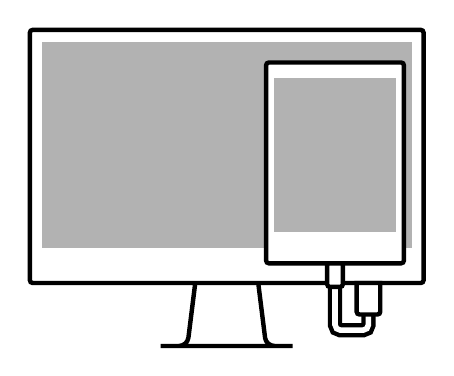
\begin{tikzpicture}[ultra thick]
    % Monitor
    \newcommand\monitorwidth{5}
    \newcommand\monitorheight{9*\monitorwidth/14}
    \newcommand\monitorborder{.15}

    \coordinate (monitor-bl) at (-3, -.25);
    \coordinate (monitor-tr) at ($(monitor-bl)+(\monitorwidth, \monitorheight)$);
    \path let \p1 = (monitor-tr), \p2 = (monitor-bl) in
        (.5 * \x1 + .5 * \x2, \y2) coordinate (monitor-b);

    \newcommand\supportback{1}
    \newcommand\supportheight{0.8}
    \newcommand\supporttop{0.8}
    \newcommand\supportbase{1.8}

    \draw[border, fill=white]
        ($(monitor-b)+(-.5 * \supporttop, 0)$)
        {[rounded corners=3]
        -- ($(monitor-b)+(-.5 * \supportback, -\supportheight)$)
        -- ($(monitor-b)+(-.5 * \supportbase, -\supportheight)$)
        -- ($(monitor-b)+(.5 * \supportbase, -\supportheight)$)
        -- ($(monitor-b)+(.5 * \supportback, -\supportheight)$)}
        -- ($(monitor-b)+(.5 * \supporttop, 0)$);

    \draw[
        border, fill=white,
        rounded corners=1,
    ] (monitor-bl) rectangle (monitor-tr);

    \fill[screen]
        (monitor-bl) ++(\monitorborder, 3 * \monitorborder)
        coordinate (monitor-screen-bl)
        rectangle ++(
            \monitorwidth - 2 * \monitorborder,
            \monitorheight - 4 * \monitorborder
        )
        coordinate (monitor-screen-tr);

    % Tablet
    \definehighlightoption{UpperKey}{border}{}
    \definehighlightoption{HomeKey}{none}{border}

    \tikzset{
        back slate/.style={
            border, fill=white,
            rounded corners=1,
        },
        lower key/.style={
            draw=border, rectangle,
            rounded corners=0.25,
            minimum width={2 * \outborder cm},
            minimum height={2 * \outborder cm},
            inner sep=0pt,
        },
        upper key/.style={
            fill=\UpperKeyFillColor, rectangle,
            rounded corners=0.25,
            minimum width={2 * \outborder cm},
            minimum height=2pt,
            yshift=-.25pt,
            inner sep=0pt,
        },
    }

    \draw[back slate] (0, 0) rectangle (\width, \height);

    \fill[screen]
        (\outborder, 4 * \outborder)
        coordinate (screen-bl)
        rectangle (\width - \outborder, \height - 2 * \outborder)
        coordinate (screen-tr);

    \coordinate (screen-c) at ($(screen-bl)!.5!(screen-tr)$);

    % Cable
    \path (.5 * \width, 0) coordinate (device-port);
    \path (monitor-bl-|monitor-tr) ++(-.7, 0) coordinate (monitor-port);

    \draw[
        border, rounded corners=2,
        double, double distance=2,
    ]
        (monitor-port) ++(0, -.4)
        |- ++(-.2, -.2)
        -| ($(device-port)+(0, -.7)$)
        -- ++(0, .4);

    \draw[border, fill=white]
        (device-port) ++(-.1, 0)
        -- ++(.2, 0) {[rounded corners=1]
        -- ++(0, -.3)
        -- ++(-.2, 0)}
        -- cycle;

    \draw[border, fill=white]
        (monitor-port) ++(.15, 0)
        {[rounded corners=1]
        -- ++(0, -.4)
        -- ++(-.3, 0)}
        -- ++(0, .4)
        -- cycle;
\end{tikzpicture}
\end{document}
